% !TEX encoding = UTF-8 Unicode
\documentclass{beamer}
% \usetheme{Luebeck}
\usetheme{Frankfurt}
\usecolortheme{default}
\setbeamercolor{bibliography entry author}{fg=black}
\beamertemplatenavigationsymbolsempty

\usepackage[english,serbian]{babel}
\usepackage[utf8]{inputenc}
\usepackage{color}
\usepackage{url}
\usepackage{graphicx}
\usepackage{amsmath}
\usepackage{amsfonts}
\graphicspath{ {images/} }

\DeclareMathOperator*{\argmax}{argmax}

\title{Automatsko prepoznavanje govora}
\subtitle{Seminarski rad u okviru kursa\\Metodologija stručnog i naučnog rada}
\author[Vladimir Vuksanović, Aleksa Kojadinović, Lazar Čeliković]{
  \texorpdfstring{Vladimir Vuksanović, vladevuksan99@gmail.com\\Aleksa Kojadinović, kojadinovic.aleksa98@gmail.com\\Lazar Čeliković, celikoviclazar@hotmail.com}
  {Vladimir Vuksanović, Aleksa Kojadinović, Lazar Čeliković}
}
\institute{Matematički fakultet}
\date{\today}

\begin{document}

\frame{\titlepage}

\begin{frame}{Sadržaj}
  \tableofcontents[hideallsubsections]
\end{frame}

\section{Uvod}
\begin{frame}
  \frametitle{Uvod}

  \begin{itemize}
    \item \textbf{Automatsko prepoznavanje govora} (eng.~{\em Automatic Speech Recognition, ASR}) je proces pretvaranja zvučnog signala govora u odgovarajući niz reči pomoću računara
    \item Neke od najznačajnijih primena su:
    \begin{itemize}
      \item pametni lični asistenti (Google Assistant, Apple Siri, \dots)
      \item transkripcija i pretraživanje audio sadržaja
      \item automatsko titlovanje snimaka
      \item pristupačnost (eng.~{\em accessibilty})
    \end{itemize} 
  \end{itemize}
\end{frame}

\section{Izazovi}
\begin{frame}
  \frametitle{Izazovi}

  \begin{enumerate}
    \item Mala količina podataka za trening
    \item Stil govora
    \begin{itemize}
      \item Izolovane reči
      \item Povezane reči
      \item Neprekidan govor
      \item Spontani govor
    \end{itemize}
    \item Karakteristike govornika (pol, starost, brzina govora...)
    \item Okruženje govornika (pozadinska buka, oprema za snimanje)
    \item Veličina rečnika
  \end{enumerate}
\end{frame}

\section{Statistički model}

\subsection{Statistički model}
\begin{frame}
  \frametitle{Statistički model}

  \begin{itemize}
    \item Koriste statističke metode za određivanje najverovatnije transkripcije
    \item Ako je $X$ ulazni zvuk, traži se najverovatniji niz reči $\hat{W} \approx \argmax_{W,S} P(X|S) P(S|W) P(W)$
  \end{itemize}

  \begin{figure}
    \begin{center}
    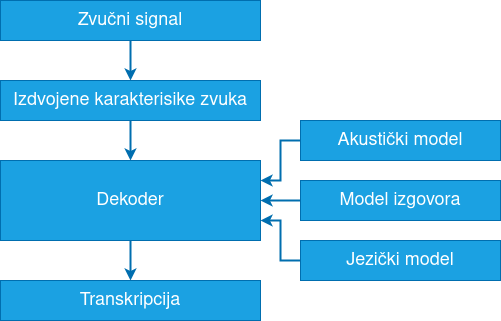
\includegraphics[scale=0.39]{statistical_model.png}
    \end{center}
    \caption{Struktura statističkog modela}
  \end{figure}
\end{frame}

\subsection{Akustički model i model izgovora}
\begin{frame}
  \frametitle{Akustički model i model izgovora}

  \begin{itemize}
    \item Akustički model 
    \begin{itemize}
      \item Predviđa verovatnoće koliko ulazni zvuk odgovara nizu fonema
      \item Foneme su najmanje jezičke jedinice na osnovu kojih mogu da se razlikuju značenja većih jedinica
      \item Implementiran skrivenim Markovljevim modelom
    \end{itemize}
    \item Model izgovora
    \begin{itemize}
      \item Mapira reči u njihov način izgovora (fonetski zapis)
      \item Definisan od strane eksperta za jezik
      \item Određuje način povezivanja modela fonema u model reči
    \end{itemize}
  \end{itemize}

  \begin{figure}
    \begin{center}
    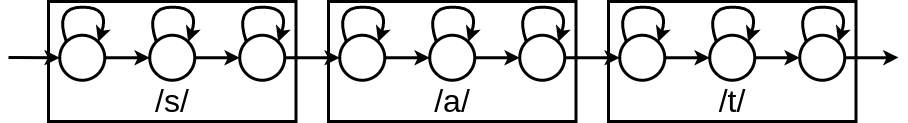
\includegraphics[scale=0.3]{word_hmm.png}
    \end{center}
    \caption{Primer skrivenog Markovljenog modela za reč ``sat''}
  \end{figure}
\end{frame}

\subsection{Jezički model}
\begin{frame}
  \frametitle{Jezički model}

  \begin{itemize}
    \item Određuje verovatnoću predviđanja rečenice na osnovu:
    \begin{itemize}
      \item relativne učestalosti reči
      \item redosleda reči
      \item sintaksne ispravnosti
      \item semantičke ispravnosti
    \end{itemize}
    \item Implementiran pomoću n-grama
    \item Dužina n-grama je obično 3 i smanjuje se dok se ne pronađe prvo pojavljivanje u trening skupu
  \end{itemize}
\end{frame}

\section{End-to-end model}

\subsection{End-to-end model}
\begin{frame}
  \frametitle{End-to-end model}
  \cite{graves2006ctc}
  \cite{chan2015las}
\end{frame}

\subsection{CTC (Connectionist Temporal Classification)}
\begin{frame}
  \frametitle{CTC (Connectionist Temporal Classification)}
\end{frame}

\subsection{Modeli zasnovani na pažnji}
\begin{frame}
  \frametitle{Modeli zasnovani na pažnji}
\end{frame}

\section{Metrike za evaluaciju}
\begin{frame}
  \frametitle{Word Error Rate (WER)}

  \begin{equation*}
    WER = \frac{I + D + S}{N}
  \end{equation*}
  gde je:
  \begin{itemize}
    \item $I$ broj umetnutih reči
    \item $D$ broj obrisanih reči
    \item $S$ broj zamenjenih reči
    \item $N$ ukupan broj reči u referenci
  \end{itemize}
\end{frame}

\section{Literatura}
\begin{frame}{Literatura}
    \bibliography{presentation} 
    \bibliographystyle{ieeetr}
\end{frame}

\end{document}